%%%%%%%%%%%%%%%%%%%%%%%%%%%%%%%%%%%%%%%%%
% Beamer Presentation
% LaTeX Template
% Version 1.0 (10/11/12)
%
% This template has been downloaded from:
% http://www.LaTeXTemplates.com
%
% License:
% CC BY-NC-SA 3.0 (http://creativecommons.org/licenses/by-nc-sa/3.0/)
%
%%%%%%%%%%%%%%%%%%%%%%%%%%%%%%%%%%%%%%%%%

%----------------------------------------------------------------------------------------
%	PACKAGES AND THEMES
%----------------------------------------------------------------------------------------

\documentclass{beamer}

\mode<presentation> {

% The Beamer class comes with a number of default slide themes
% which change the colors and layouts of slides. Below this is a list
% of all the themes, uncomment each in turn to see what they look like.

%\usetheme{default}
%\usetheme{AnnArbor}
%\usetheme{Antibes}
%\usetheme{Bergen}
%\usetheme{Berkeley} %with Outline
%\usetheme{Berlin}
%\usetheme{Boadilla}
\usetheme{CambridgeUS} %This is well-looking
%\usetheme{Copenhagen}
%\usetheme{Darmstadt}
%\usetheme{Dresden}
%\usetheme{Frankfurt}
%\usetheme{Goettingen}
%\usetheme{Hannover}
%\usetheme{Ilmenau}
%\usetheme{JuanLesPins}
%\usetheme{Luebeck}
%\usetheme{Madrid}
%\usetheme{Malmoe}
%\usetheme{Marburg}
%\usetheme{Montpellier}
%\usetheme{PaloAlto}
%\usetheme{Pittsburgh}
%\usetheme{Rochester}
%\usetheme{Singapore}
%\usetheme{Szeged}
%\usetheme{Warsaw}

% As well as themes, the Beamer class has a number of color themes
% for any slide theme. Uncomment each of these in turn to see how it
% changes the colors of your current slide theme.

%\usecolortheme{albatross}
%\usecolortheme{beaver}
%\usecolortheme{beetle}
%\usecolortheme{crane}
\usecolortheme{dolphin}
%\usecolortheme{dove}
%\usecolortheme{fly}
%\usecolortheme{lily}
%\usecolortheme{orchid}
%\usecolortheme{rose}
%\usecolortheme{seagull}
%\usecolortheme{seahorse}
%\usecolortheme{whale}
%\usecolortheme{wolverine}

%\setbeamertemplate{footline} % To remove the footer line in all slides uncomment this line
%\setbeamertemplate{footline}[page number] % To replace the footer line in all slides with a simple slide count uncomment this line

%\setbeamertemplate{navigation symbols}{} % To remove the navigation symbols from the bottom of all slides uncomment this line
}

\usepackage{graphicx} % Allows including images
\usepackage{booktabs} % Allows the use of \toprule, \midrule and \bottomrule in tables
\usepackage{amsmath, amssymb, amsfonts}
\usepackage{mathrsfs}
\usepackage{amsthm}
%----------------------------------------------------------------------------------------
%	TITLE PAGE
%----------------------------------------------------------------------------------------

\title[VE216]{VE216 Recitation Class 7} % The short title appears at the bottom of every slide, the full title is only on the title page

\author{ZHU Yilun} % Your name
\institute[SJTU] % Your institution as it will appear on the bottom of every slide, may be shorthand to save space
{
UM-SJTU Joint Institute \\ % Your institution for the title page
\medskip
\textit{VE216 SU20 TA Group} % Your email address
}
\date{2020 Summer} % Date, can be changed to a custom date e.g.:\today

\begin{document}

\begin{frame}
\titlepage % Print the title page as the first slide
\end{frame}

\begin{frame}
\frametitle{Overview} % Table of contents slide, comment this block out to remove it
\tableofcontents % Throughout your presentation, if you choose to use \section{} and \subsection{} commands, these will automatically be printed on this slide as an overview of your presentation
\end{frame}

%----------------------------------------------------------------------------------------
%	PRESENTATION SLIDES
%----------------------------------------------------------------------------------------

\begin{frame}
    \frametitle{Before we start}
    \begin{itemize}
        \item To me, concept of convolution, FS, FT are ``theoretically inspiring''
        \item Now we turn to applications like 
        \begin{itemize}
            \item filtering (Chap. 6)
            \item sampling (Chap. 7)
            \item communication (Chap. 8)
        \end{itemize}
        which are ``practically inspiring''
        \item What's even more amazing is that all these applications depend on only two properties: 
        \begin{itemize}
            \item Convolution Property: \[f_1(t)* f_2(t) \stackrel{\mathscr{F}}{\longleftrightarrow} F_1(\omega) \cdot F_2(\omega)    \]
            \item Time-domain Multiplication: \[f_1(t)\cdot f_2(t) \stackrel{\mathscr{F}}{\longleftrightarrow} \frac{1}{2 \pi} F_1(\omega) * F_2(\omega)    \]
        \end{itemize}
    \end{itemize}
\end{frame}


%------------------------------------------------
\section{Chapter 6: Filtering}
%------------------------------------------------
\begin{frame}
\frametitle{Filtering}
\begin{itemize}
\item Convolution Property: $h(t)* x(t) \stackrel{\mathscr{F}}{\longleftrightarrow} H(\omega) X(\omega)    $

\begin{figure}
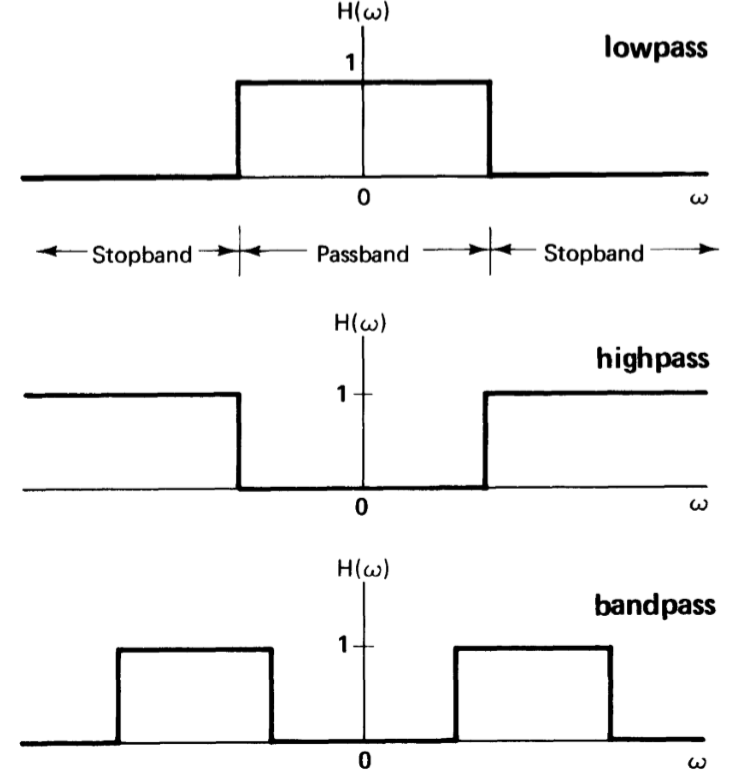
\includegraphics[width=0.5\linewidth]{filter}
\end{figure}
\item LTI systems can be viewed as ``filters'' in frequency domain
\end{itemize}
\end{frame}

\begin{frame}[t]
    \frametitle{Exercise - Filtering}
    \begin{figure}
        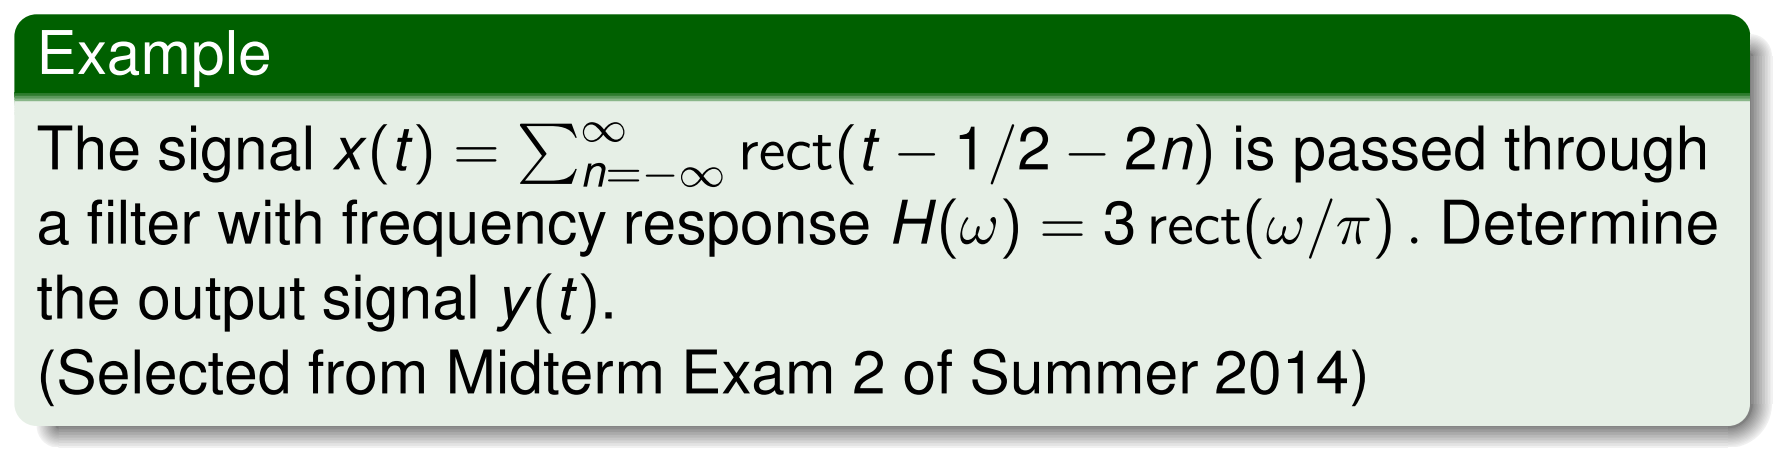
\includegraphics[width=0.8\linewidth]{ex_filter}
    \end{figure}
\end{frame}


%------------------------------------------------------
\section{Chapter 7: Sampling}
%------------------------------------------------------

\begin{frame}
    \frametitle{Overview of DSP}
    \begin{figure}
        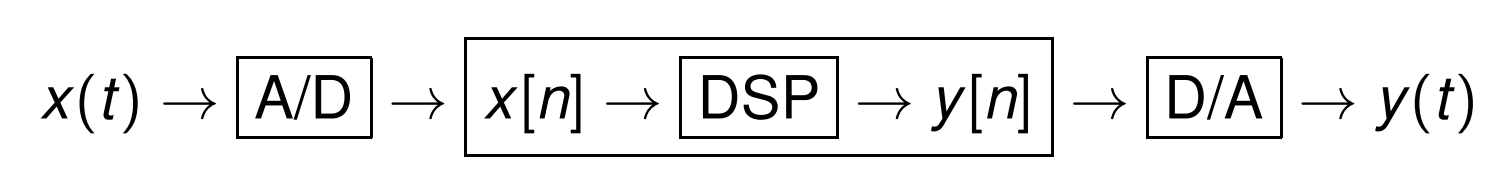
\includegraphics[width=0.8\linewidth]{dsp}
    \end{figure}
    \begin{itemize}
        \item Why DSP? Only way possible, Computers, low price, etc 
        \item Here we only focus on the left and right part. (DSP will be discussed in VE351)
        \item We want to show that processing the discrete-time signal (the samples) is equivalent to processing the continuous-time signal (the initial signal).
        \item Time-domain Multiplication: \[f_1(t)\cdot f_2(t) \stackrel{\mathscr{F}}{\longleftrightarrow} \frac{1}{2 \pi} F_1(\omega) * F_2(\omega)    \]
    \end{itemize}
\end{frame}

\subsection{Sampling Theorem}



\begin{frame}
\frametitle{Sampling Theorem}
\begin{figure}
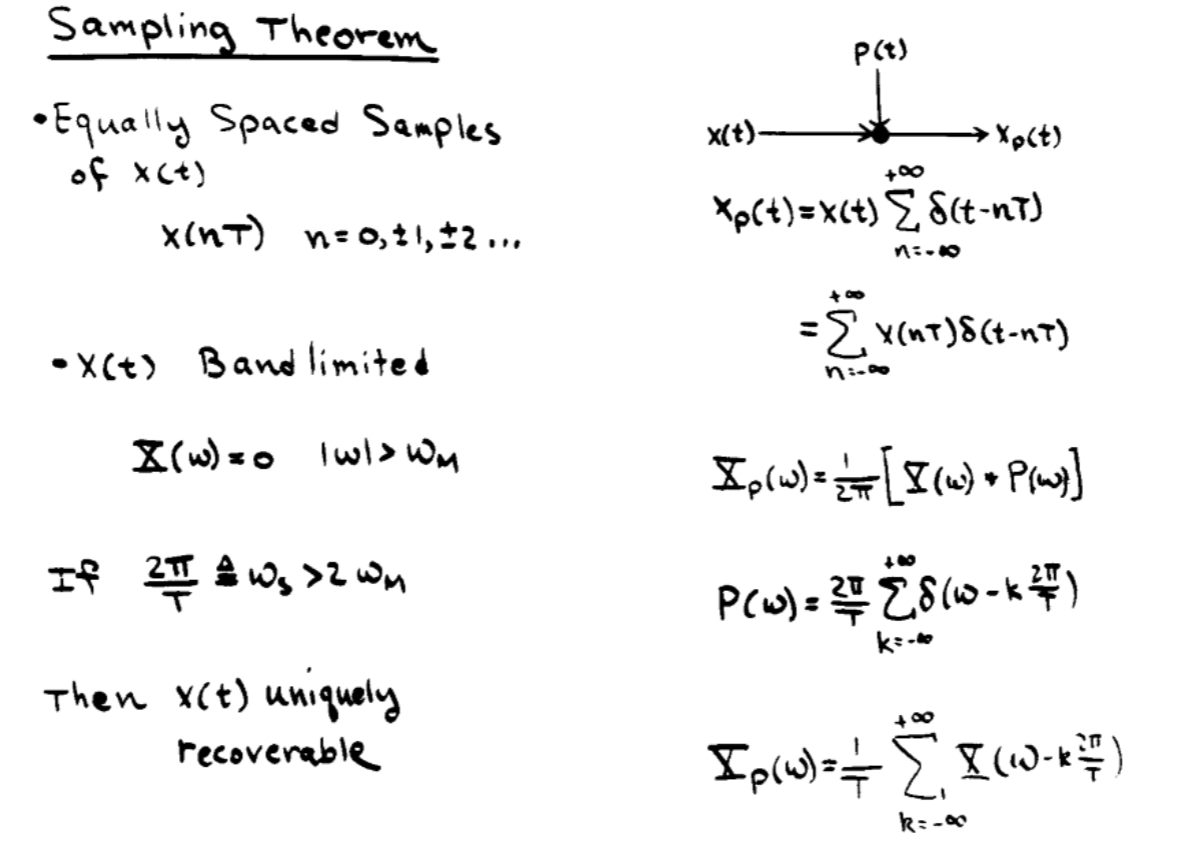
\includegraphics[width=0.8\linewidth]{sample1}
\end{figure}
\end{frame}

\begin{frame}
\frametitle{Recoverable}
\begin{figure}
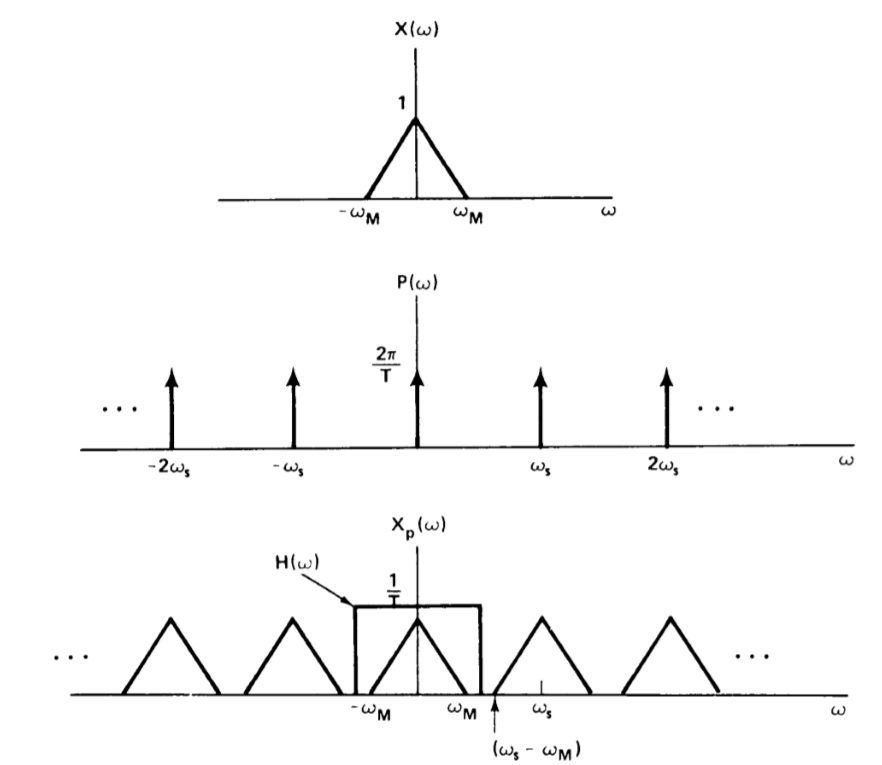
\includegraphics[width=0.7\linewidth]{sample2}
\end{figure}
\end{frame}

\begin{frame}
\frametitle{Aliasing}
\begin{figure}
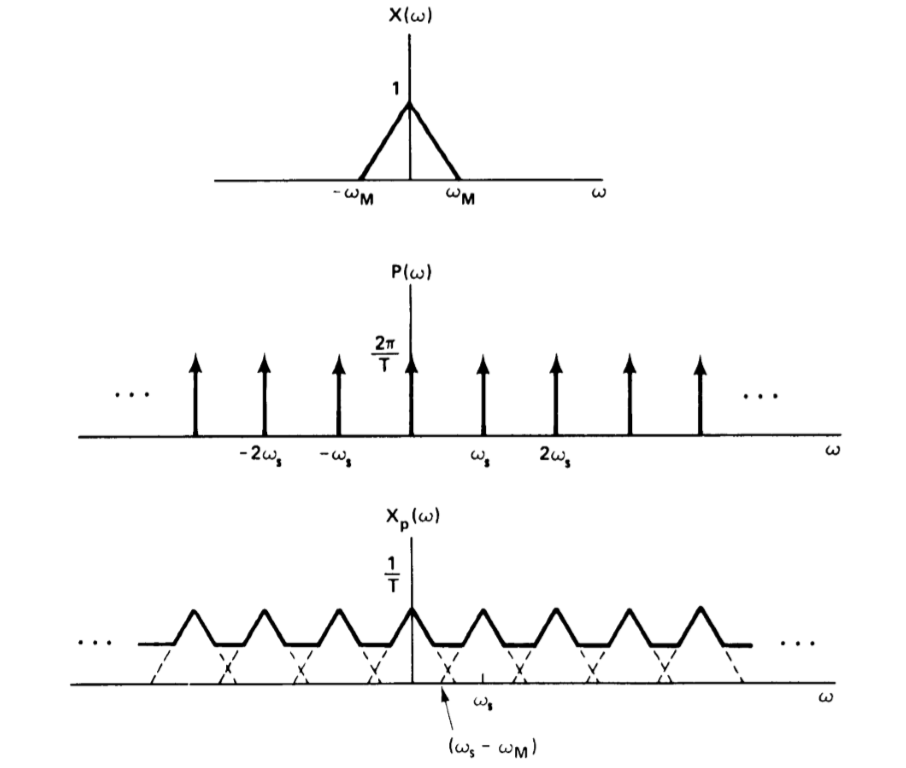
\includegraphics[width=0.7\linewidth]{sample3}
\end{figure}
\end{frame}

\begin{frame}
    \frametitle{Nyquist rate - interpretation}
    \begin{figure}
    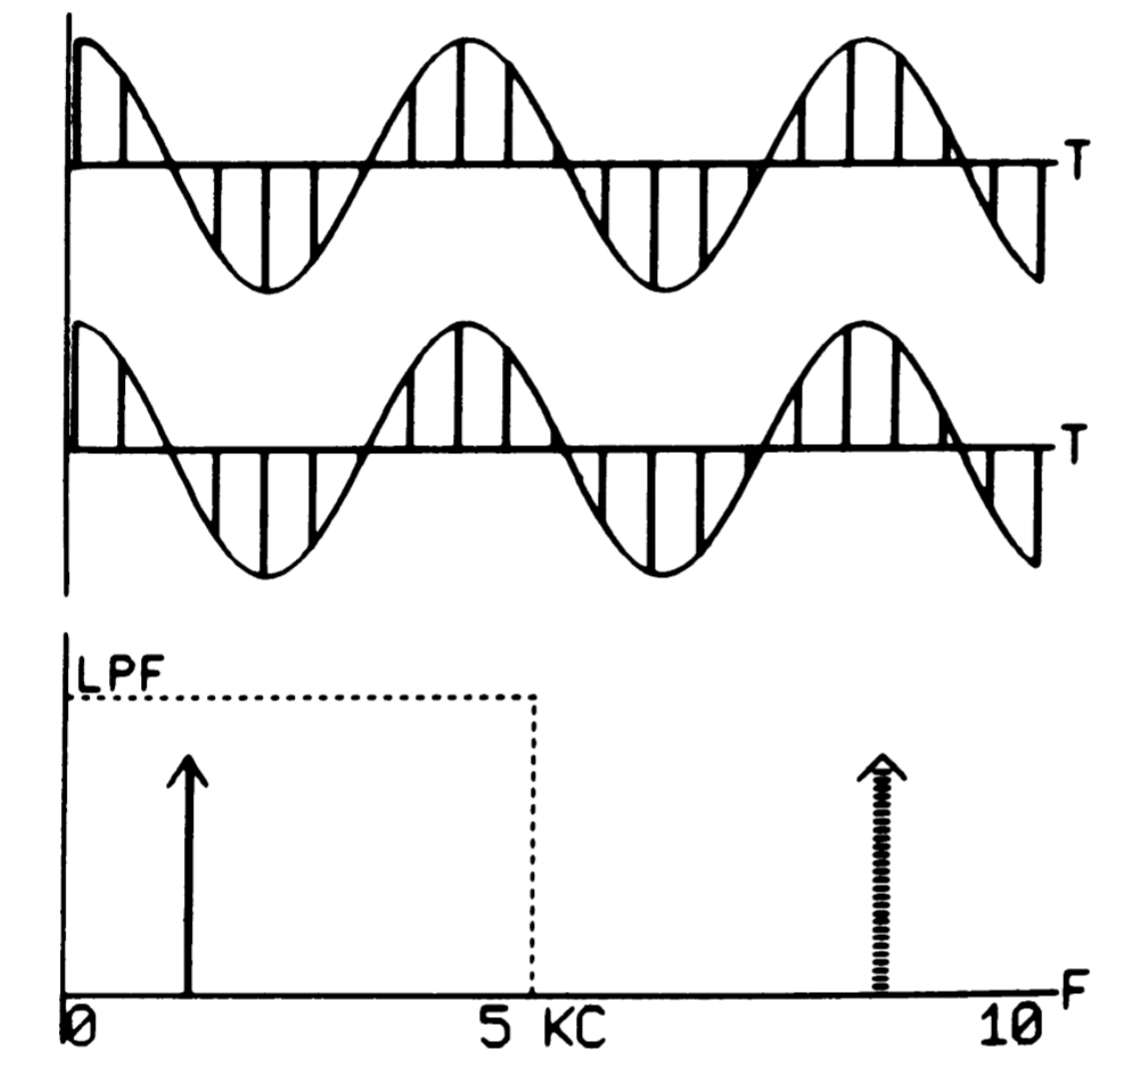
\includegraphics[width=0.5\linewidth]{cos_sample}
    \end{figure}
\begin{itemize}
    \item Interpretation: at least 2 samples in a period
    \item Information lost during sampling? Consider const. signal.
\end{itemize}
\end{frame}



\begin{frame}[t]
    \frametitle{Another way to understand Sampling: relation with FS}
    \begin{figure}
        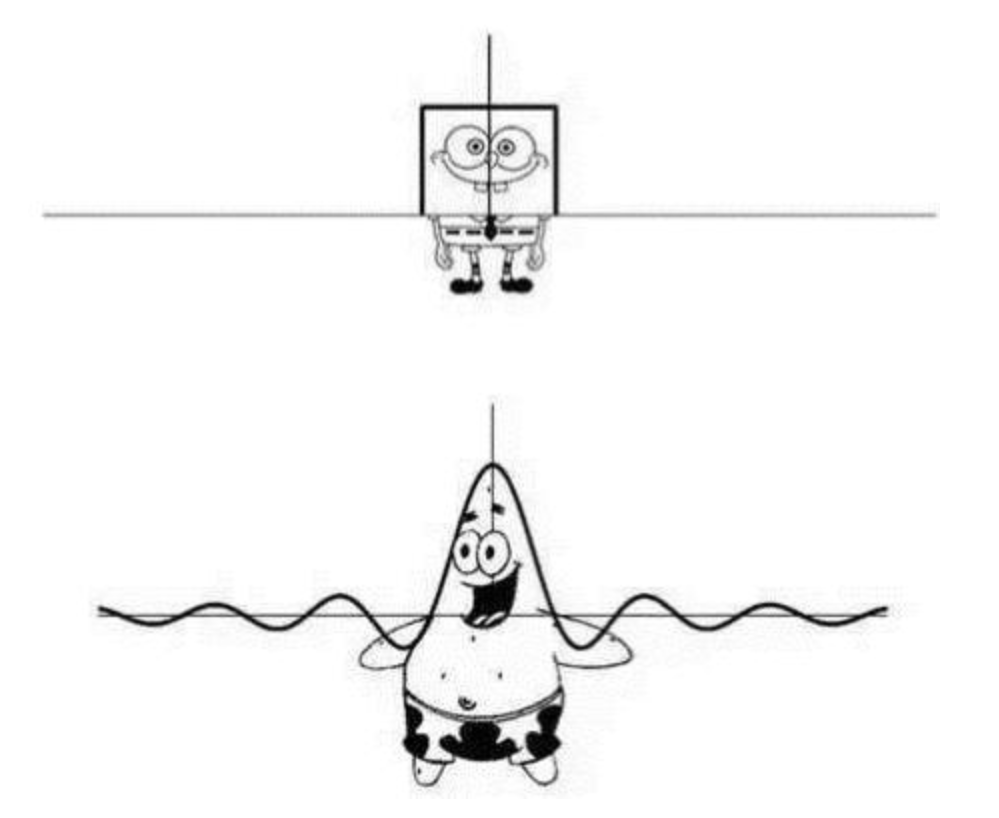
\includegraphics[width=0.4\linewidth]{sponge.PNG}
    \end{figure}
    \begin{center}
        \begin{align*}
            \text{Patrick Star} &\stackrel{FT}{\longleftrightarrow}  \text{SpongeBob SquarePants} \\[0.5em]
            \text{Periodic SpongeBob SquarePants} &\stackrel{FS / FT}{\longleftrightarrow}  \text{Samples of Patrick Star} \\[0.5em]  
            \text{Samples of Patrick Star } &\stackrel{FT}{\longleftrightarrow}  \text{Periodic SpongeBob SquarePants}       
        \end{align*}
    \end{center} 
\end{frame}



\begin{frame}
\frametitle{Sampling $\&$ Reconstruction}
\begin{figure}
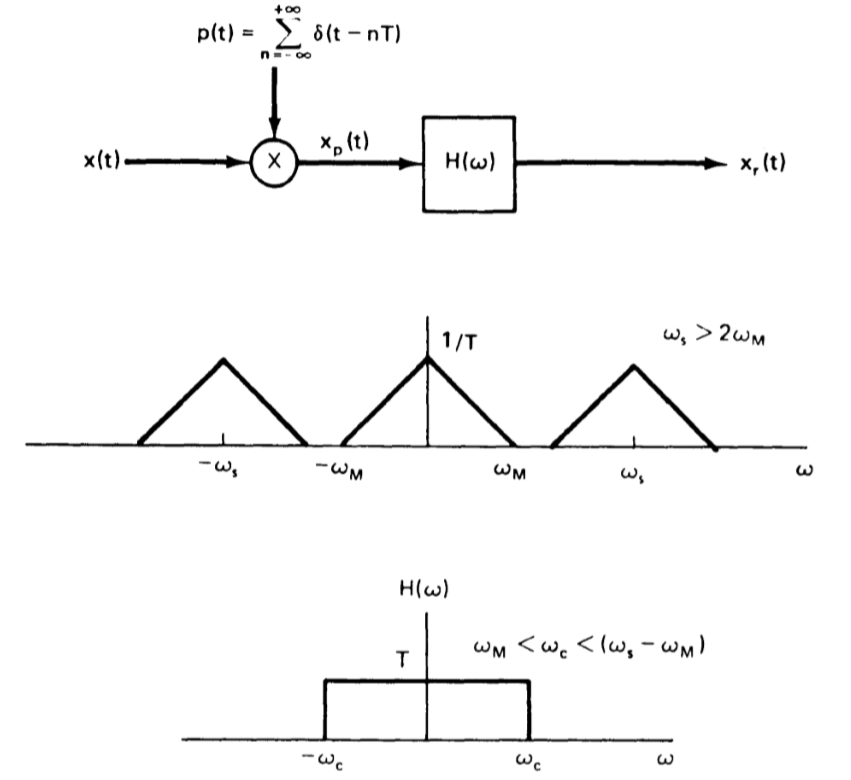
\includegraphics[width=0.6\linewidth]{sample4}
\end{figure}
\end{frame}


%-------------------------------------------------
\section{Conclusion}
\begin{frame}
\frametitle{Conclusion}
\begin{itemize}
\item The concept of sampling itself is motivating - consider eye (watching the wheels) and ear (ultrasonic)
\item Sampling is closely related with reconstruction, which will be the focus of next week.
\item The place we are in the big picture.
\item For sampling-related problems, I prefer to view them graphically (often in freq. domain).
\end{itemize}
\end{frame}

%------------------------------------------------

\begin{frame}
\Huge{\centerline{The End}}
\end{frame}

%----------------------------------------------------------------------------------------

\end{document} 